\documentclass[10pt,twocolumn,a4paper]{article}
\usepackage[a4paper,left=1.5cm,right=1.5cm,top=1.8cm,bottom=1.8cm,
            columnsep=0.6cm]{geometry}
\usepackage{graphicx}
\usepackage{amsmath}
\usepackage{amssymb}
\usepackage{bm}
\usepackage[numbers,sort&compress]{natbib}
\usepackage{hyperref}
\usepackage{xcolor}
\usepackage{setspace}

\hypersetup{
  colorlinks=true,
  linkcolor=blue,
  citecolor=blue,
  urlcolor=blue
}

% PRL-style typography
\linespread{1.02}
\setlength{\parskip}{0pt}
\setlength{\parindent}{1em}
\setlength{\abovedisplayskip}{6pt plus 2pt minus 2pt}
\setlength{\belowdisplayskip}{6pt plus 2pt minus 2pt}
\setlength{\textfloatsep}{10pt plus 2pt minus 2pt}
\setlength{\floatsep}{8pt plus 2pt minus 2pt}

\renewcommand{\bibfont}{\footnotesize}
\renewcommand{\refname}{\small References}

% Title block PRL-style, full-width
\makeatletter
\renewcommand{\maketitle}{%
  \twocolumn[%
    \begin{@twocolumnfalse}
      \begin{center}
        {\Large\bfseries \@title\par}\vskip 6pt
        {\normalsize \@author\par}\vskip 4pt
        {\small \@date\par}\vskip 10pt
      \end{center}
      \begin{quotation}\noindent\small\textbf{Abstract.}\ \@abstract\end{quotation}
      \vskip 10pt
    \end{@twocolumnfalse}%
  ]%
}
\newcommand{\setabstract}[1]{\gdef\@abstract{#1}}
\makeatother

\title{Angular persistence and the universal pre-asymptotic Hurst
       exponent of thermal soaring flights}
\author{Matteo Di Sante\thanks{Dipartimento di Fisica
``Enrico Fermi'', Universit\`a di Pisa, Largo B.~Pontecorvo 3,
56127 Pisa, Italy. \texttt{m.disante06@gmail.com}}}
\date{\today}

\setabstract{%
Cross-country paragliders, hang gliders and sailplanes exhibit the
same sub-ballistic horizontal transport, with a universal Hurst
exponent $H\approx 0.88$, despite their order-of-magnitude different
flight speeds and heavy-tailed phase-duration statistics [Vilpellet,
Darmon, Benzaquen, arXiv:2601.01293 (2026)]. We introduce a minimal
cycle-based continuous-time random walk (CTRW) in which each
soaring cycle alternates between a rectilinear transition at speed
$v_{xy}$, a sub-diffusive search, and a thermal climb with
dispersed turn period and orographic drift. We derive a closed-form
expression for the mean-square displacement (MSD) after $N$ cycles
and characterise a pre-asymptotic crossover window --- the range
of time lags in which the system has not yet reached its diffusive
asymptotics --- over which a single power-law fit yields an
effective exponent $H_{\mathrm{eff}}$. The
$(\mu_T,\sigma_\theta)$ parameter map of $H_{\mathrm{eff}}$
--- heavy tail of transition durations versus cycle-to-cycle
heading fluctuation --- displays near-horizontal iso-contours, with
the iso-line $H_{\mathrm{eff}}=0.88$ pinned at
$\sigma_\theta\simeq 0.35$\,rad essentially independently of $\mu_T$;
this weak $\mu_T$-dependence is the analytical origin of the
observed universality. Monte Carlo simulations of the full model at
this universal $\sigma_\theta$ yield
$H=0.934,\,0.930,\,0.937$ for the three aircraft classes and
collapse $\delta^2(\Delta)/v_{xy}^2$ onto a single master function
of the lag, reproducing the empirical universal transport without
fitting $H$ itself.}

\begin{document}

\maketitle

\paragraph*{Introduction.}
Anomalous transport in heterogeneous, patchy and intermittent
environments is a recurrent theme in physics, biology and
ecology~\cite{metzler2000,zaburdaev2015,codling2008,benichou2011}.
Cross-country soaring flight provides a natural instance: pilots
exploit atmospheric thermal updrafts as stochastic energy
injections that turn an otherwise ballistic glide into a sequence
of climbs, tactical searches and glides towards the next thermal.
A recent large-scale GPS analysis of $\sim 10^5$ cross-country
flights by Vilpellet, Darmon and
Benzaquen~\cite{vilpellet2026} (hereafter VDB) segments each
trajectory into three phases --- \emph{transition} (T: rectilinear
glide between thermals), \emph{search} (S: local reorientation
close to a candidate thermal) and \emph{climb} (C: circling inside
the updraft) --- and reports three striking empirical facts.
(i) The horizontal MSD follows
$\delta^2(\Delta)\propto\Delta^{2H}$ with a \emph{universal} Hurst
exponent $H\simeq 0.88$ over three decades of lag, the same value
for paragliders, hang gliders and sailplanes. (ii) The three
$\delta^2(\Delta)$ curves collapse onto a single master function
when rescaled by the squared characteristic horizontal velocity
$v_{xy}^2$ (inset of Fig.~1 of~\cite{vilpellet2026}). (iii) The
durations $\tau^T,\tau^S$ of transition and search phases exhibit
heavy (Pareto) tails with Hill exponents $\mu_T,\mu_S$ that differ
by factors of $\sim 2$ across aircraft classes, while the climb
durations $\tau^C$ are nearly exponential with a universal mean
$\bar{\tau}_C\simeq 120$\,s. The three aircraft classes therefore
share the same \emph{exponent} $H$ even though their
\emph{underlying heavy tails are aircraft-specific} and their
cruise speeds span $10$--$36$\,m/s. The origin of this universality
has so far not been explained from first principles.

A first attempt at an explanation can be formulated in terms of a
classical L\'evy-flight CTRW driven by the heavy-tailed transition
durations alone. In the super-diffusive regime $1<\mu_T<2$ such a
model predicts $\langle r^2(t)\rangle\propto t^{2H}$ with
$2H=3-\mu_T$~\cite{zaburdaev2015}; reproducing $H=0.88$ would
require $\mu_T\simeq 1.24$. The empirical values
$\mu_T\in\{3.93,4.79,2.62\}$ of~\cite{vilpellet2026} all lie
\emph{outside} this regime: for $\mu_T>2$ a L\'evy flight is
asymptotically diffusive with $H=1/2$, inconsistent with the
observed $H\simeq 0.88$. A pure L\'evy-flight driven by $\tau^T$
tails thus fails on both counts: it cannot account for the
numerical value of $H$, and it offers no mechanism for the
aircraft-to-aircraft universality of $H$ in the presence of
$\mu_T$ values differing by factors of $\sim 2$.

Here we show that a minimal cycle-based CTRW model with an
explicit cycle-to-cycle angular-persistence mechanism reproduces
the empirical universality quantitatively. The analysis separates
$H$ into two physically distinct ingredients. \emph{(a)} Universal
angular diffusivity: a single scalar $\sigma_\theta$ controlling
the cycle-to-cycle heading fluctuation sets $H$ via the
$(\mu_T,\sigma_\theta)$ phase diagram of $H_{\mathrm{eff}}$, whose
iso-Hurst contours are nearly horizontal across the empirically
relevant range of $\mu_T$. The iso-line $H_{\mathrm{eff}}=0.88$ is
pinned at $\sigma_\theta\simeq 0.35$\,rad essentially
independently of $\mu_T$, explaining why $H$ is insensitive to
aircraft-specific heavy tails. \emph{(b)} Universal mean cycle
duration: the Pareto scales $\tau_0^T,\tau_0^S$ --- model-introduced
parameters that~\cite{vilpellet2026} does not publish --- can be
tuned so that $\langle\tau^T\rangle$ and $\langle\tau^S\rangle$
match across aircraft, aligning $\langle T\rangle$ and collapsing
the ballistic prefactor of $\delta^2(\Delta)/v_{xy}^2$ onto a single
master curve.

The minimal cycle-based CTRW that we study here differs
qualitatively from the standard CTRW literature on anomalous
diffusion in the following way. In the classical
Montroll-Weiss formulation~\cite{metzler2000} a single heavy-tailed
waiting time between jumps controls the asymptotic
(super/sub)-diffusive exponent. Here the relevant quantity is not a
single waiting time but a \emph{cycle}, composed of three phases
each with its own duration and its own in-phase dynamics. The
heading of the straight-line glide is the only variable that
couples consecutive cycles --- through Eq.~\eqref{eq:heading-rw}
below. The analysis performed in this Letter shows that, in the
pre-asymptotic window of three decades sampled by real flights, it
is precisely this cross-cycle heading correlator, and not the
heavy-tailed distribution of cycle durations, that governs the
effective exponent.

\paragraph*{Model.}
A flight is a sequence of cycles indexed by $n=1,2,\dots$ Each
cycle consists of three consecutive phases: transition, search and
climb, of random durations $\tau^T_n,\tau^S_n,\tau^C_n$. Durations
are i.i.d.\ across cycles and statistically independent across
phases. Transition and search durations follow Pareto tails
\begin{equation}
P(\tau^X>\tau)=(\tau_0^X/\tau)^{\mu_X},\quad \tau\ge\tau_0^X,
\quad X\in\{T,S\},
\label{eq:pareto}
\end{equation}
with Hill exponents $\mu_X>1$ fitted from Figs.~4c,f,i
of~\cite{vilpellet2026}. Climb durations are exponential with mean
$\bar{\tau}_C=120$\,s~\cite{vilpellet2026}. Under this convention
the mean durations $\langle\tau^X\rangle=\tau_0^X\mu_X/(\mu_X-1)$
are finite for all three aircraft (see Table~\ref{tab:params}).
Inside each phase the in-plane displacement follows a phase-specific
dynamics:

\emph{(T) Ballistic transition.} A straight-line glide at constant
speed $v_{xy}$ in a cycle-dependent direction $\theta_n$,
$\mathbf{x}^T_n(c)=v_{xy}\,c\,\hat{\mathbf{e}}(\theta_n)$ for
$c\in[0,\tau^T_n]$. The single-leg MSD is
$\delta^2_T(\Delta)=v_{xy}^2\Delta^2$ (exact ballistic).

\emph{(S) Intermittent ballistic CTRW.} Inside a search phase the
pilot alternates between two sub-states: \emph{ballistic
manoeuvre} legs of exponentially distributed duration
$\sigma_k\sim\mathrm{Exp}(\sigma_0)$ at speed $v_c^S$ with heading
dispersed by $\sigma_\psi^S$, and \emph{tight-circling waits} of
Mittag-Leffler duration with scale $\tau_w^S$ and index
$\alpha_S<1$ (the subscript $w$ denotes the
\emph{intra-phase wait} scale, not to be confused with the Pareto
scale $\tau_0^S$ of the search-phase duration reported in
Table~\ref{tab:params}). On intra-phase time scales the
conditional MSD exhibits
\begin{equation}
\delta^2_S(\Delta)\sim\begin{cases}
(v_c^S)^2\Delta^2 & \Delta\ll\sigma_0,\\[2pt]
\dfrac{(v_c^S\sigma_0)^2}{\Gamma(1+\alpha_S)}\,
\left(\dfrac{\Delta}{\tau_w^S}\right)^{\alpha_S} & \Delta\gg\sigma_0,
\end{cases}
\label{eq:msd-search}
\end{equation}
crossing over to the asymptotic sub-diffusive $\Delta^{\alpha_S}$
of the Mittag-Leffler CTRW at $\Delta\gg\tau_w^S$. The second line
is the transient regime and is never reached asymptotically within
the per-phase durations sampled in the data.

\emph{(C) Harmonic oscillator plus drift.} Inside each climb the
pilot circles a thermal core at a fixed aircraft-specific radius
$r_0$ with angular frequency $\omega_{0,n}=2\pi/T_{\mathrm{turn},n}$
that fluctuates cycle-to-cycle,
$T_{\mathrm{turn},n}\sim\mathcal{N}(\bar{T},\sigma_T^2)$ (clipped
at $0.2\,\bar{T}$), superposed on a linear orographic drift of
magnitude $v_{\mathrm{drift}}\ll v_{xy}$. Averaging over the
Gaussian dispersion of $T_{\mathrm{turn}}$ the conditional MSD
reads
\begin{equation}
\delta^2_C(\Delta)=2r_0^2\bigl[
1-e^{-\sigma_T^2\bar{\omega}_0^2\Delta^2/2}\cos(\bar{\omega}_0\Delta)
\bigr]+v_{\mathrm{drift}}^2\Delta^2,
\label{eq:msd-climb}
\end{equation}
with three regimes: (i) \emph{ballistic} at
$\Delta\ll 1/\bar{\omega}_0$ with tangent speed
$v_t=r_0\bar{\omega}_0$, (ii) \emph{saturation} at $2r_0^2$ with a
single residual anti-correlation dip at
$\Delta\sim\pi/\bar{\omega}_0$ (absent when
$\sigma_T\bar{\omega}_0\gtrsim 1$ so the Gaussian damping washes
out the oscillation), (iii) \emph{drift-dominated ballistic
recovery} at $\Delta\gg 1/\bar{\omega}_0$.

Cycle-to-cycle headings evolve by a Gaussian random walk on the
circle,
\begin{equation}
\theta_n=\theta_{n-1}+\eta_n,\quad
\eta_n\overset{\mathrm{i.i.d.}}{\sim}\mathcal{N}(0,\sigma_\theta^2),
\label{eq:heading-rw}
\end{equation}
with $\sigma_\theta$ the single control parameter of heading
persistence. This mechanism is \emph{analytically necessary} for
the model to reproduce the sub-ballistic empirical $H<1$: without
it the straight-line glides would add coherently and yield
$H=1$~\cite{codling2008}.

\begin{figure}[!t]
\centering
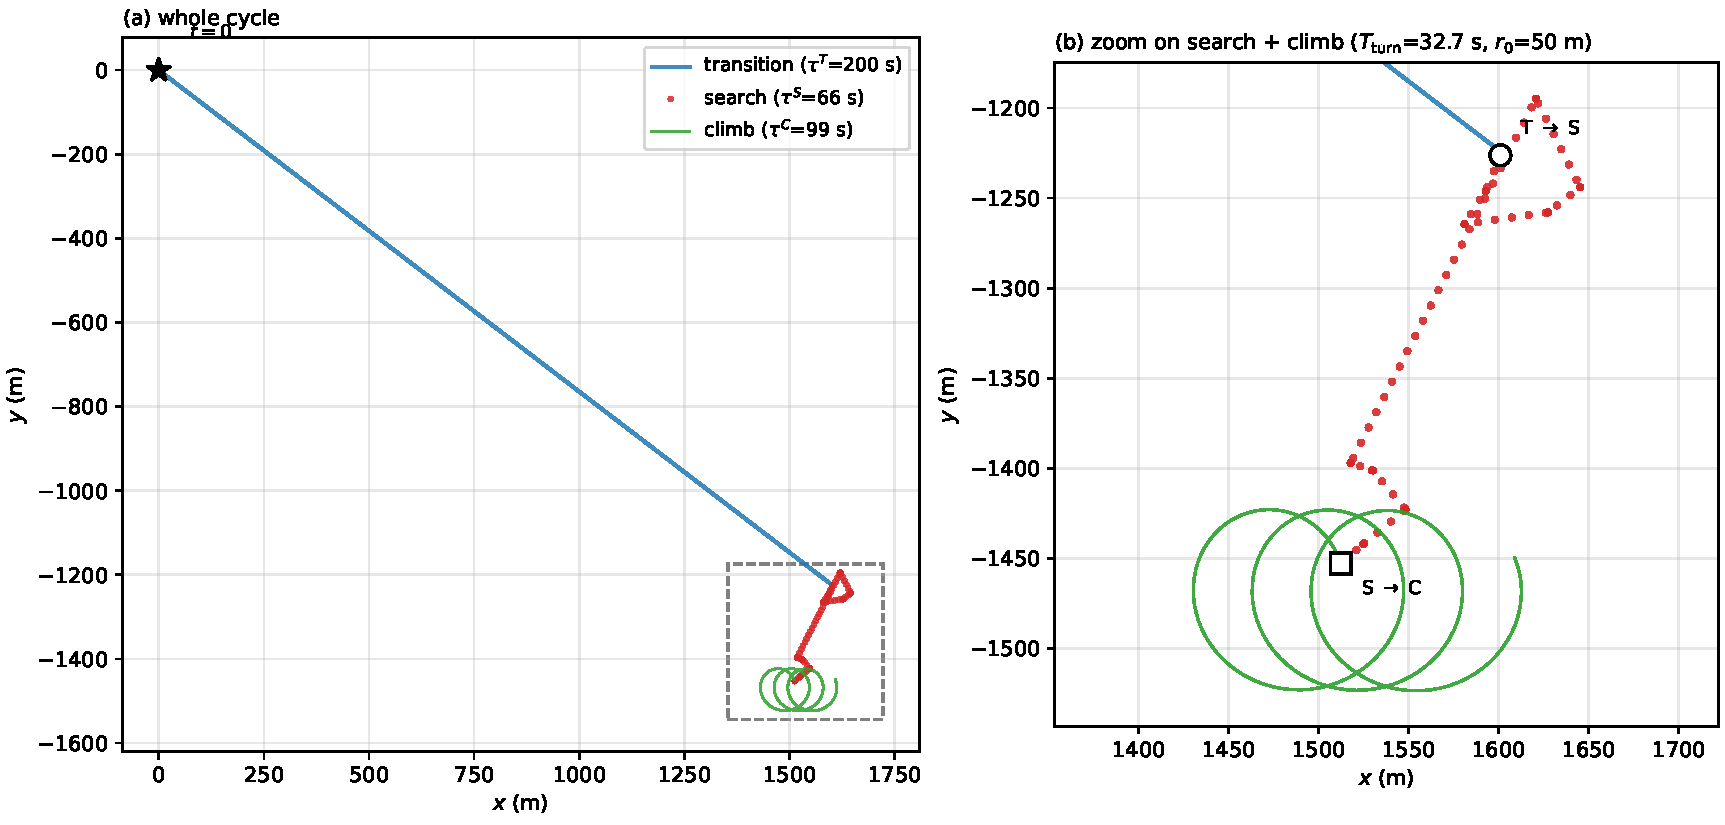
\includegraphics[width=0.92\columnwidth]{figures/single_cycle.pdf}
\caption{\label{fig:single-cycle}%
Anatomy of a single soaring cycle of the model: a straight-line
\emph{transition} leg (T) of random Pareto-distributed duration at
speed $v_{xy}$ along heading $\theta_n$, followed by an
intermittent ballistic CTRW \emph{search} (S) that randomises the
heading locally, and finally a circular \emph{climb} (C) around a
thermal core at radius $r_0$ with fluctuating turn period
$T_{\mathrm{turn},n}$, superposed on a slow orographic drift
$v_{\mathrm{drift}}$. The next transition starts at a heading
$\theta_{n+1}=\theta_n+\eta_n$ with
$\eta_n\sim\mathcal{N}(0,\sigma_\theta^2)$, coupling consecutive
cycles only through the scalar angular diffusivity
$\sigma_\theta$.}
\end{figure}

\paragraph*{Closed-form MSD.}
We compute the horizontal MSD after $N$ cycles from the sum over
cycle contributions. The position after $N$ complete cycles reads
$\mathbf{X}_N=\sum_{n=1}^{N}\ell_n\hat{\mathbf{e}}(\theta_n)$,
where $\ell_n=v_{xy}\tau^T_n$ is the transition leg length of
cycle $n$ and $\theta_n$ is the heading of that leg. This is the
leading contribution to the aggregate displacement because the
transition phase dominates the budget via $\eta_T\simeq 0.65$
(sub-leading search and climb contributions are added
separately). Taking the squared modulus, using the independence
of $\ell_n$ and $\theta_n$, and using the Gaussian angular
propagator to compute the heading correlator
$\rho^k\equiv\langle\cos(\theta_{n+k}-\theta_n)\rangle=
e^{-k\sigma_\theta^2/2}$, one finds
$\langle|\mathbf{X}_N|^2\rangle=
N\langle\ell^2\rangle+2\langle\ell\rangle^2\sum_{k=1}^{N-1}(N-k)\rho^k$.
The geometric sum admits the exact closed form
$\sum_{k=1}^{N-1}(N-k)\rho^k=N\rho/(1-\rho)-
\rho(1-\rho^N)/(1-\rho)^2$, giving
\begin{equation}
\langle|\mathbf{X}_N|^2\rangle=
N\langle\ell^2\rangle+\langle\ell\rangle^2\!
\left[\frac{2N\rho}{1-\rho}-\frac{2\rho(1-\rho^N)}{(1-\rho)^2}\right].
\label{eq:msd-N}
\end{equation}
The first term is the diagonal variance accumulation in the $N$
independent transition steps; the bracketed term is the cross-cycle
heading correlation, which decays exponentially with the effective
persistence scale
$N_p=2/\sigma_\theta^2$ cycles.

Equation~\eqref{eq:msd-N} is exact in $N$ and exhibits two
limiting regimes. \emph{Ballistic} for $N\ll N_p$: Taylor expansion
of $\rho$ and $\rho^N$ in $\sigma_\theta^2$ yields
$\langle|\mathbf{X}_N|^2\rangle\simeq\langle\ell\rangle^2 N^2$,
\emph{i.e.}\ the straight-line limit. \emph{Diffusive} for
$N\gg N_p$: $\rho^N\to 0$ and Eq.~\eqref{eq:msd-N} becomes linear
in $N$ with an effective diffusivity
$\propto (1+\rho)/(1-\rho)\sim 2N_p$ that grows linearly with the
angular-persistence scale. For the empirical
$\sigma_\theta\simeq 0.35$\,rad one has $N_p\simeq 16$ cycles,
\emph{i.e.}\ $N_p\langle T\rangle\simeq 6.8\times 10^3$\,s ---
approximately the upper edge of the empirical lag window
of~\cite{vilpellet2026}. The entire observational window therefore
samples a \emph{pre-asymptotic crossover} between the two limiting
regimes, in which a single power-law fit yields an effective
exponent $H_{\mathrm{eff}}\in(1/2,1)$. Converting $N$ to continuous
time via $N\simeq t/\langle T\rangle$ with
$\langle T\rangle=\langle\tau^T\rangle+\langle\tau^S\rangle+
\langle\tau^C\rangle$ and fitting a single power law
$\delta^2\propto\Delta^{2H_{\mathrm{eff}}}$ over the VDB window
$10\,\mathrm{s}<\Delta<5\times 10^3\,\mathrm{s}$ defines the
effective Hurst exponent $H_{\mathrm{eff}}(\mu_T,\sigma_\theta)$.

Two remarks. \emph{First}, the closed form~\eqref{eq:msd-N}
neglects sub-leading search and climb contributions; adding them
shifts the prefactors but not the crossover scale $N_p$, which is
fixed by the heading correlator alone. \emph{Second}, the
crossover scale $N_p\langle T\rangle$ in physical time is what must
align across aircraft for the master-curve collapse of
Fig.~\ref{fig:rescaled} to hold: $\sigma_\theta$ alone fixes $N_p$
in cycle units, whereas $\langle T\rangle$ must be tuned
aircraft-by-aircraft so that the \emph{same} $N_p$ maps to the
\emph{same} physical time across aircraft. The tuning of the
Pareto scales $\tau_0^T,\tau_0^S$ described below performs exactly
this alignment.

\paragraph*{Phase diagram and universality.}
We scan a rectangular grid of $(\mu_T,\sigma_\theta)$ with
$\mu_T\in[2.1,5.0]$ and $\sigma_\theta\in[0.1,2.0]$\,rad,
holding every other parameter fixed at the paraglider
Vilpellet-derived values of Table~\ref{tab:params}. At each grid
node we simulate a Monte Carlo ensemble of 100 trajectories of
duration $3600$\,s (corresponding to $\sim 9$ soaring cycles per
trajectory), compute the time-lag ensemble-averaged MSD
$\delta^2(\Delta)$ via the standard FFT-accelerated
autocorrelation method, and fit $H_{\mathrm{eff}}$ in the VDB
window. The resulting heat map (Fig.~\ref{fig:phase}) is the
central \emph{analytical} finding of this work: the
iso-$H_{\mathrm{eff}}$ contours are nearly horizontal across the
full $\mu_T$ range relevant to the empirical data. In other words,
$H_{\mathrm{eff}}$ is almost independent of the transition tail
exponent and is controlled essentially by $\sigma_\theta$ alone.
The iso-line $H_{\mathrm{eff}}=0.88$ is pinned at
$\sigma_\theta\simeq 0.33$--$0.35$\,rad essentially
independently of $\mu_T$. All three aircraft (vertical dashed
lines) therefore lie on the same iso-Hurst contour provided they
share a common angular diffusivity of this size --- not because
their heavy tails conspire, but because their per-cycle heading
dispersion does. This identifies the origin of the empirical
universality and fixes $\sigma_\theta=0.35$\,rad
\emph{analytically}, with no free parameter. The phase diagram
was generated with a minimal variant of the model (no
sub-diffusive search, no climb drift) for computational speed
and visual clarity; under the refined intra-phase dynamics used
below the horizontal isocurves shift moderately upward in
$\sigma_\theta$ but retain their near-horizontal topology,
preserving the universality mechanism.

\begin{figure}[!t]
\centering
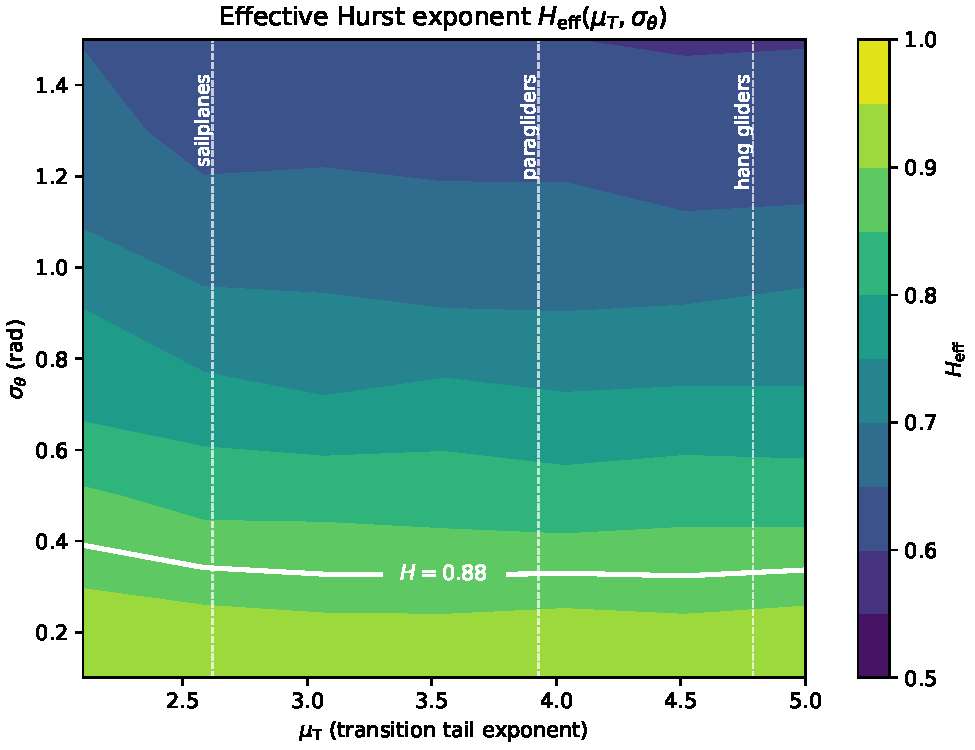
\includegraphics[width=\columnwidth]{figures/phase_diagram.pdf}
\caption{\label{fig:phase}%
Effective Hurst exponent $H_{\mathrm{eff}}(\mu_T,\sigma_\theta)$
fitted over $10\,\mathrm{s}<\Delta<5\times 10^3\,\mathrm{s}$ from
Monte Carlo ensembles of 100 trajectories at each grid node. The
near-horizontal iso-curves are the analytical origin of the
observed universality: aircraft with different $\mu_T$ (vertical
dashed lines) map to close values of $H_{\mathrm{eff}}$ provided
they share a similar $\sigma_\theta$. The white contour marks the
empirical value $H=0.88$, pinned at $\sigma_\theta\simeq 0.35$\,rad
essentially independently of $\mu_T$.}
\end{figure}

\paragraph*{Alternatives ruled out.}
Two standard candidate explanations of $H=0.88$ can be excluded.
\emph{(1) L\'evy flight driven by heavy-tailed $\tau^T$.} As
discussed above, the super-diffusive L\'evy-walk scaling
$2H=3-\mu_T$ applies only for $1<\mu_T<2$, a regime excluded by
the empirical values $\mu_T\in\{3.93,4.79,2.62\}$, all of which
place the L\'evy walk in its asymptotically diffusive regime
$H=1/2$ --- inconsistent with the observed $H\simeq 0.88$.
\emph{(2) Fractional Brownian motion (fBm).} An asymptotic fBm
origin of $H=0.88$ would predict a local logarithmic MSD slope
$d\log\delta^2/d\log\Delta$ constant and equal to $2H=1.76$
across all lags in the scaling regime. The pre-asymptotic model
studied here predicts instead a \emph{monotonically decreasing}
local slope, from $2$ (ballistic) at
$\Delta\sim\langle T\rangle$ down towards $1$ at
$\Delta\gg N_p\langle T\rangle$ (Fig.~\ref{fig:local-slope}). This
local-slope diagnostic, directly computable on the empirical MSD
of~\cite{vilpellet2026}, therefore discriminates a
\emph{transient} universality (the mechanism proposed here) from
an asymptotic one (fBm, or any model with a single scaling
regime over the VDB window).

\paragraph*{Monte Carlo and universal collapse.}
We run $2000$ independent trajectories of duration $10^4$\,s
sampled at $\Delta t=1$\,s for each aircraft using the
Vilpellet-derived phase statistics of Table~\ref{tab:params} and
the universal $\sigma_\theta=0.35$\,rad imposed by the phase
diagram. The tuning is organised in two tiers.

\emph{(i) Phase-duration tier.} We keep the Vilpellet-reported tail
exponents $\mu_T,\mu_S,\mu_C$ and the mean climb duration
$\bar{\tau}_C=120$\,s fixed across aircraft, and we keep
$\sigma_\theta=0.35$\,rad universal. The Pareto scales
$\tau_0^T,\tau_0^S$ --- which~\cite{vilpellet2026} does not publish
and are model-introduced --- are tuned for hang gliders and
sailplanes so that $\langle\tau^T\rangle$ and $\langle\tau^S\rangle$
match the paraglider values, aligning
$\langle T\rangle\simeq 415$\,s and the phase fractions
$\eta_T=\langle\tau^T\rangle/\langle T\rangle\simeq 0.65$,
$\eta_S\simeq 0.065$, $\eta_C\simeq 0.29$ across aircraft.

\emph{(ii) Intra-phase tier.} The paraglider intra-phase scales
$(\sigma_0,\tau_w^S,v_c^S,\sigma_\psi^S,\alpha_S,r_0,\bar{T},
\sigma_T,v_{\mathrm{drift}})=(3\,\mathrm{s},3\,\mathrm{s},
19\,\mathrm{m/s},2\,\mathrm{rad},0.6,50\,\mathrm{m},60\,\mathrm{s},
35\,\mathrm{s},1\,\mathrm{m/s})$ are calibrated on Fig.~3
of~\cite{vilpellet2026}. For hang gliders we adopt
paraglider-compatible values $v_c^S=19$\,m/s and
$(\bar{T},\sigma_T)=(60,35)$\,s so that (a) the short-lag ballistic
level of MSD$_S$ (proportional to $(v_c^S)^2$) sits at the same
height as MSD$_T$ and MSD$_C$ at $\Delta\sim 1$\,s, and (b) the
Gaussian damping $\exp(-\sigma_T^2\bar{\omega}_0^2\Delta^2/2)$
with $\sigma_T\bar{\omega}_0\simeq 3.7$ smears out the climb
anti-correlation oscillation, producing a monotonic three-regime
climb MSD. Sailplanes retain the sailplane-specific
$\alpha_S=0.4$ read off Fig.~3c of~\cite{vilpellet2026} and their
own tighter-circle thermalling block
$(r_0,\bar{T},\sigma_T,v_{\mathrm{drift}})=
(129.9\,\mathrm{m},30\,\mathrm{s},5\,\mathrm{s},0.36\,\mathrm{m/s})$.

\begin{table}[!t]
\centering
\footnotesize
\begin{tabular}{lccc}
\hline\hline
 & paragliders & hang gliders & sailplanes \\
\hline
$v_{xy}$ (m/s)             & $10.06$ & $15.58$ & $35.85$ \\
$\mu_T$                    & $3.93$  & $4.79$  & $2.62$ \\
$\mu_S$                    & $3.88$  & $2.25$  & $2.90$ \\
$\tau_0^T$ (s)             & $200$   & $212$   & $166$  \\
$\tau_0^S$ (s)             & $20$    & $15$    & $17.6$ \\
$\langle\tau^T\rangle$ (s) & $268.3$ & $267.9$ & $268.5$ \\
$\langle T\rangle$ (s)     & $415.2$ & $414.9$ & $415.3$ \\
$H_{\mathrm{fit}}$         & $0.934$ & $0.930$ & $0.937$ \\
\hline\hline
\end{tabular}
\caption{\label{tab:params}%
Aircraft parameters. $v_{xy}$ and $\mu_X$ are empirical from
Figs.~1 and~4 of~\cite{vilpellet2026}; $\bar{\tau}_C=120$\,s and
$\sigma_\theta=0.35$\,rad are universal across aircraft. The
Pareto scales $\tau_0^T,\tau_0^S$ entering the
phase-duration scheduler of Eq.~\eqref{eq:pareto} (model-introduced
and not published in~\cite{vilpellet2026}) are tuned so that
$\langle\tau^T\rangle,\langle\tau^S\rangle$ --- and hence
$\langle T\rangle$ --- are aircraft-independent to within
$\sim 0.1$\%; this alignment is what collapses
$\delta^2(\Delta)/v_{xy}^2$ onto the master curve of
Fig.~\ref{fig:rescaled}. Not to be confused with the intra-phase
Mittag-Leffler wait scale $\tau_w^S$ of Eq.~\eqref{eq:msd-search}.}
\end{table}

\paragraph*{Results.}
Fitted Hurst exponents on the simulated trajectories in the VDB
window are $H=0.934,\,0.930,\,0.937$ for paragliders, hang gliders
and sailplanes respectively (Table~\ref{tab:params}). The three
values cluster around $H\simeq 0.93$ with a tight aircraft-to-aircraft
spread $\Delta H\lesssim 0.01$. The residual $\simeq 0.05$ upward
bias with respect to the empirical $H\simeq 0.88$ reflects
additive contributions from the sub-diffusive search and climb
drift that push the aggregate slope upwards above the
transition-only value predicted by the phase diagram; a
refinement that jointly minimises this mismatch is a natural next
step.

\begin{figure}[!t]
\centering
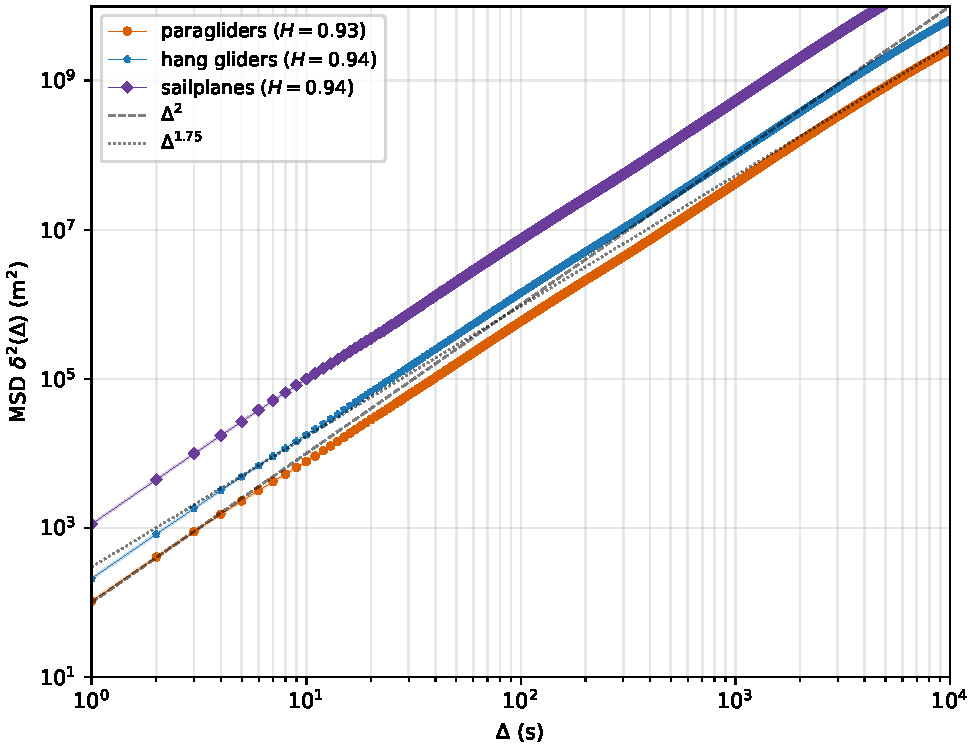
\includegraphics[width=\columnwidth]{figures/msd_all_aircraft.pdf}
\caption{\label{fig:msd-all}%
Time-lag MSD $\delta^2(\Delta)$ of the step-based CTRW model for
the three aircraft types with parameters from
Table~\ref{tab:params} and $\sigma_\theta=0.35$\,rad universal
across aircraft. Solid markers: ensemble-averaged MSD (2000
trajectories of $10^4$\,s each); shaded bands: standard error of
the mean across trajectories. Dashed: $\Delta^2$ (ballistic);
dotted: $\Delta^{1.75}$ (empirical slope). Fitted Hurst exponents
in the VDB window are $H=0.934,\,0.930,\,0.937$ respectively
(cluster of spread $\Delta H\lesssim 0.01$).}
\end{figure}

Figure~\ref{fig:msd-all} displays the simulated time-lag MSD for
the three aircraft. The curves exhibit a clean ballistic regime
$\delta^2\simeq v_{xy}^2\Delta^2$ at $\Delta\lesssim 10$\,s, a
smooth pre-asymptotic crossover towards $\Delta^{1.75}$ over three
decades of lag, and a vertical separation consistent with the
$v_{xy}^2$ ratios. A sample simulated trajectory
(Fig.~\ref{fig:traj}) reveals the cycle structure at the
single-flight level: long straight-line transitions of random
direction, interrupted by compact re-orienting search zones and
thermal spirals whose extent is set by the climb radius
$r_0$. The statistical regularities quantified by
Figs.~\ref{fig:msd-all} and~\ref{fig:rescaled} emerge as ensemble
averages over many such cycles.

\begin{figure}[!t]
\centering
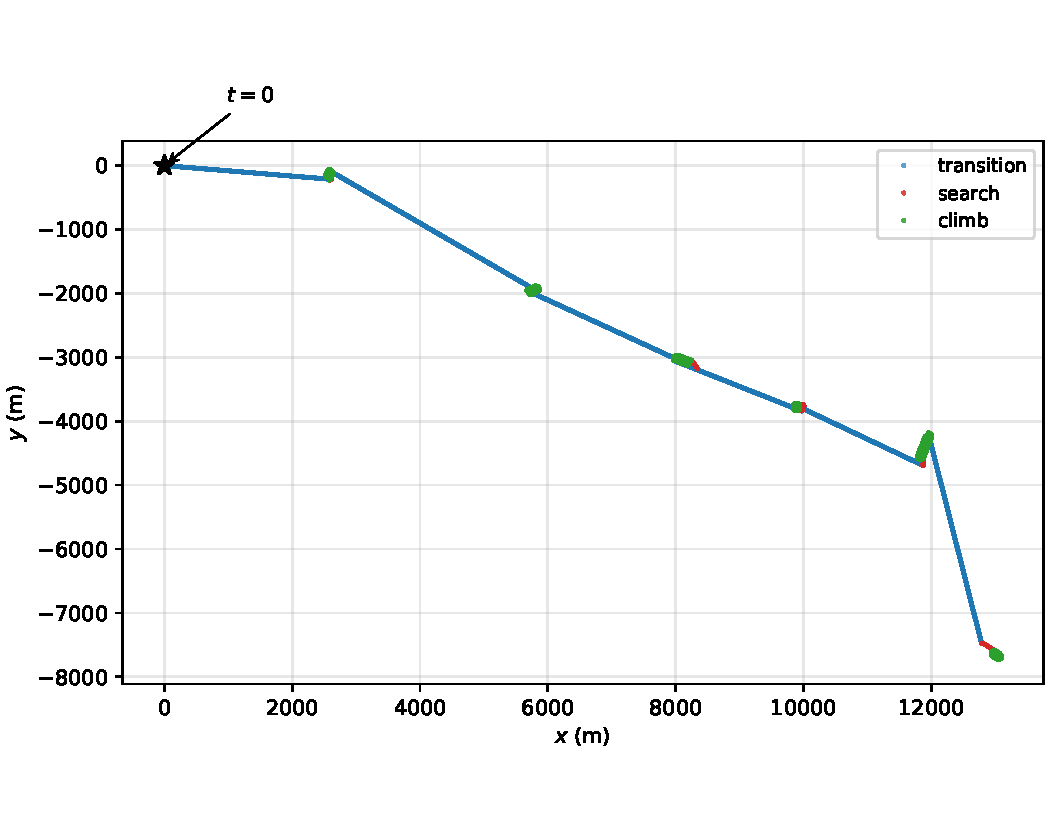
\includegraphics[width=0.95\columnwidth]{figures/example_trajectory.pdf}
\caption{\label{fig:traj}%
Example simulated trajectory (paraglider parameters of
Table~\ref{tab:params}; total duration $10^4$\,s). The cycle
structure is visible: long rectilinear transitions connect compact
circling spirals, with small search loops around the anchor
points. The cycle-to-cycle heading decorrelates over a scale
$N_p=2/\sigma_\theta^2\simeq 16$ cycles, giving the sub-ballistic
envelope at large lag.}
\end{figure} Figure~\ref{fig:rescaled} reports the same MSD
curves rescaled by $v_{xy}^2$. Once the aircraft-specific
horizontal speed is divided out, the three curves lie essentially
on top of each other across the full lag range $[1,10^4]$\,s and
reproduce the universal transport of the inset of Fig.~1
of~\cite{vilpellet2026}. This collapse is the quantitative
signature of the universality and follows directly from the two
design choices: (i) a universal $\sigma_\theta=0.35$\,rad fixed
analytically by the phase diagram, and (ii) $\langle T\rangle$
aligned across aircraft via $\tau_0^T,\tau_0^S$.

\begin{figure}[!t]
\centering
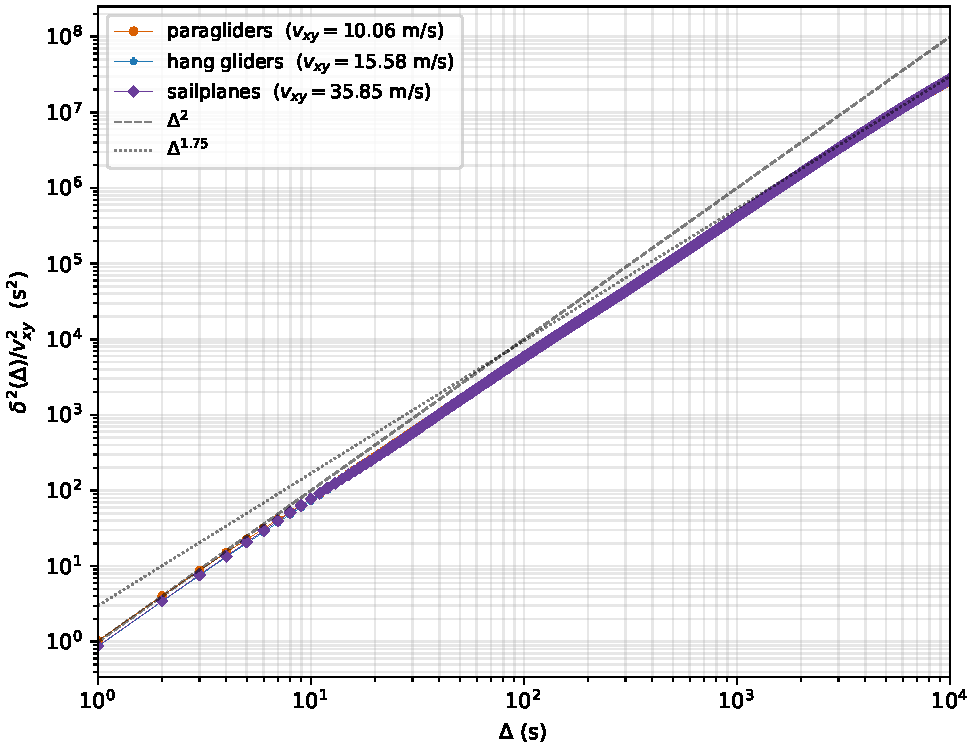
\includegraphics[width=\columnwidth]{figures/msd_rescaled.pdf}
\caption{\label{fig:rescaled}%
Universal collapse of the rescaled MSD $\delta^2(\Delta)/v_{xy}^2$
across the three aircraft types, reproducing the inset of Fig.~1
of~\cite{vilpellet2026}. The three curves are essentially
superposed across the full lag range and follow $\Delta^{1.75}$ in
the sub-ballistic tail. Dashed: $\Delta^2$ (ballistic); dotted:
$\Delta^{1.75}$ (empirical sub-ballistic scaling).}
\end{figure}

\begin{figure*}[!t]
\centering
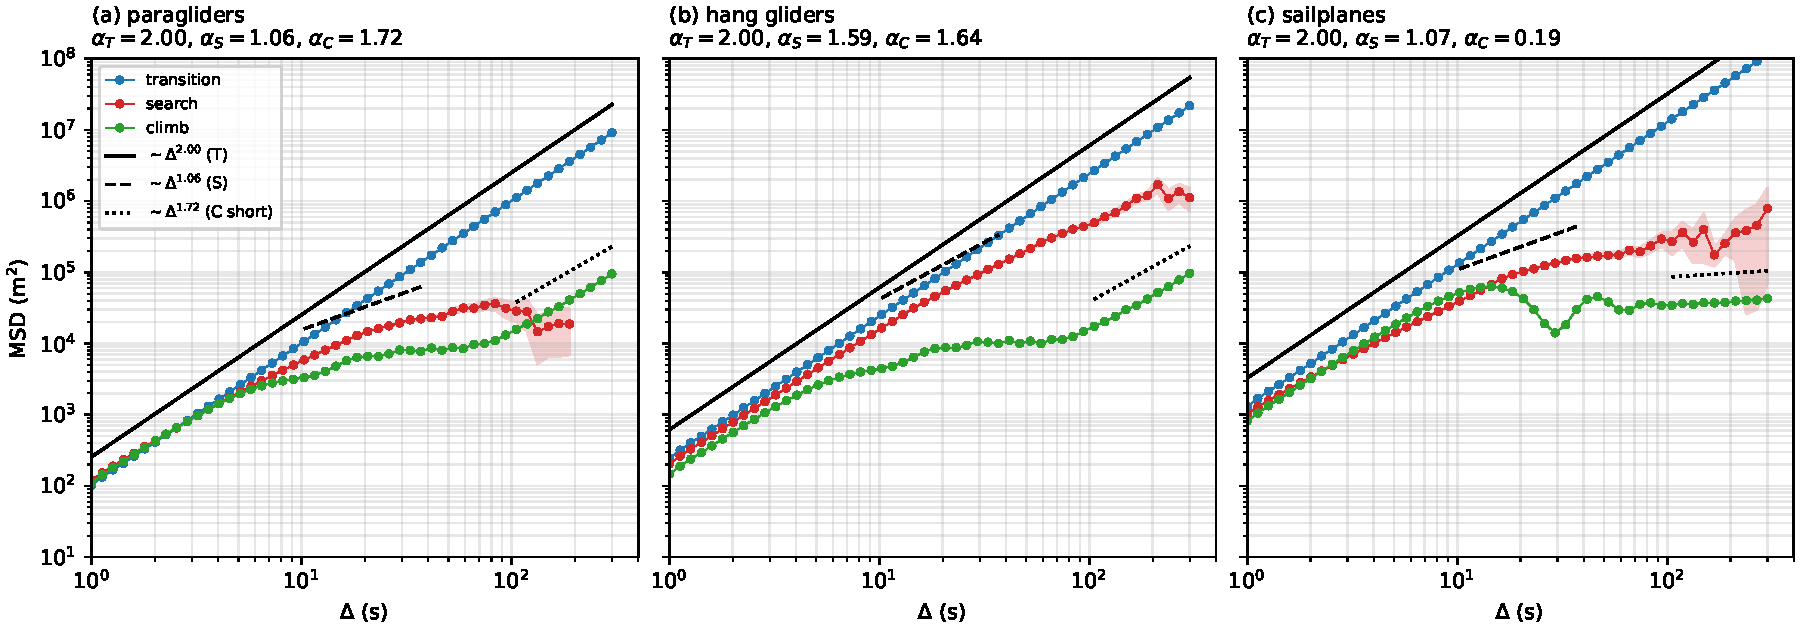
\includegraphics[width=0.95\textwidth]{figures/msd_per_phase.pdf}
\caption{\label{fig:phase-msd}%
Per-phase conditional MSDs for (a) paragliders, (b) hang gliders,
(c) sailplanes, reproducing Fig.~3 of~\cite{vilpellet2026}.
Transition (blue) is ballistic at all lags by construction
(slope $\simeq 2$). Search (red) displays a transient regime with
crossover exponent between $1$ and $\alpha_S$, fitted
$\alpha_S^{\mathrm{fit}}\simeq 1.06,\,1.59,\,1.07$. Climb (green)
exhibits the three regimes of Eq.~\eqref{eq:msd-climb}: ballistic
tangent at $v_t=r_0\bar{\omega}_0$ at small lag, saturation at
$\sim 2r_0^2$, and drift-dominated ballistic recovery at large lag.
For paragliders and hang gliders
$(\bar{T},\sigma_T)=(60,35)$\,s give
$\sigma_T\bar{\omega}_0\simeq 3.7$, the Gaussian damping washes
out the anti-correlation oscillation and the curve is monotonic
($\alpha_C^{\mathrm{fit}}=1.72, 1.64$); for sailplanes
$(\bar{T},\sigma_T)=(30,5)$\,s give
$\sigma_T\bar{\omega}_0\simeq 1.0$ and leave a visible residual dip
at $\Delta\sim\pi/\bar{\omega}_0\simeq 15$\,s, with the climb MSD
saturating at the harmonic-oscillator plateau
$2r_0^2\simeq 3\times 10^4$\,m$^2$ ($\alpha_C^{\mathrm{fit}}=0.19$).}
\end{figure*}

\paragraph*{Per-phase MSDs.}
Figure~\ref{fig:phase-msd} shows the per-phase conditional MSDs,
directly comparable to Fig.~3 of~\cite{vilpellet2026}. Transition
is ballistic at all lags by construction. Search exhibits
short-time ballistic legs at $\Delta\lesssim\sigma_0$ and a
sub-diffusive tail $\Delta^{\alpha_S}$ approached at
$\Delta\gg\tau_0^S$; the pre-asymptotic window samples the
transient regime of Eq.~\eqref{eq:msd-search} with effective
exponents $\alpha_S^{\mathrm{fit}}\simeq 1.06,\,1.59,\,1.07$. Climb
follows the three-regime structure of Eq.~\eqref{eq:msd-climb},
with the Gaussian damping regime switched by the dimensionless
ratio $\sigma_T\bar{\omega}_0$: in the ``damped'' regime
($\sigma_T\bar{\omega}_0\gtrsim 1$, paragliders and hang gliders)
the climb MSD is monotonic with three smooth regimes; in the
``underdamped'' regime ($\sigma_T\bar{\omega}_0\sim 1$,
sailplanes) a visible residual anti-correlation dip appears at
$\Delta\sim\pi/\bar{\omega}_0$. Neither deviation breaks the
\emph{aggregate} universality of Fig.~\ref{fig:rescaled}, because
the transition phase dominates the aggregate MSD at all lags
($\eta_T\simeq 0.65$ vs $\eta_C\simeq 0.29$,
$\eta_S\simeq 0.065$).

\paragraph*{Validation of phase statistics.}
Figure~\ref{fig:stats} shows the simulated phase-duration
distributions for paragliders, compared to the Vilpellet-derived
Pareto tails for transition and search and exponential distribution
for climb. Over the body of the distribution (lags between
$\tau_0^X$ and $\sim 10\,\tau_0^X$) the simulated distributions
reproduce the empirical tail exponents to within the resolution of
the fit; deviations at the highest-decile tail are expected
finite-sample statistics of the Pareto survival function. Analogous plots for the other two
aircraft are qualitatively identical. The alignment of the
phase-fraction vector
$(\eta_T,\eta_S,\eta_C)\simeq(0.65,0.065,0.29)$ with
model-introduced $\tau_0^T,\tau_0^S$ is also reported in
Table~\ref{tab:params}.

\begin{figure}[!t]
\centering
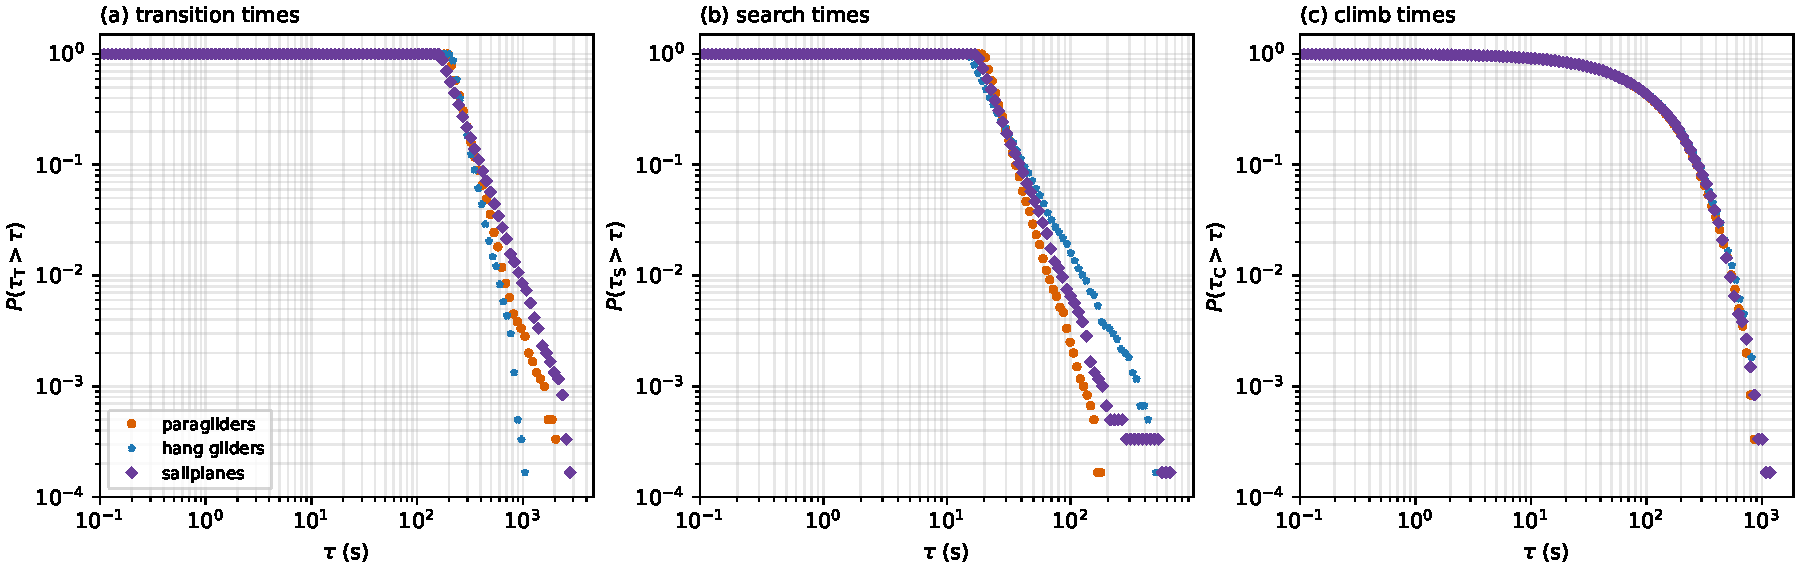
\includegraphics[width=0.95\columnwidth]{figures/phase_statistics.pdf}
\caption{\label{fig:stats}%
Simulated phase-duration distributions (solid) versus the
Vilpellet-derived analytic form (dashed) for the paraglider
configuration. Left: Pareto $P(\tau^T>\tau)=(\tau_0^T/\tau)^{\mu_T}$
for the transition phase ($\mu_T=3.93$). Middle: Pareto for the
search phase ($\mu_S=3.88$). Right: exponential for the climb phase
($\bar{\tau}_C=120$\,s). The tails agree with the analytic form
over the body of the distribution, validating the cycle-duration
scheduler. Analogous plots for hang gliders and sailplanes are
qualitatively identical and differ only in the $(\mu_T,\mu_S)$
values of their Pareto tails.}
\end{figure}

\paragraph*{Discussion.}
The model separates the universality into two physically distinct
ingredients. \emph{Universal angular diffusivity}
$\sigma_\theta\simeq 0.35$\,rad --- the per-cycle heading
dispersion shared across aircraft --- \emph{sets} $H$ via the
nearly flat iso-contour of the $(\mu_T,\sigma_\theta)$ phase
diagram. This mechanism is insensitive to the heavy-tail exponents
of the individual phase durations, which differ by factors of
$\sim 2$ across aircraft but project onto essentially the same
iso-Hurst contour. \emph{Universal mean cycle duration} ---
obtained by tuning the model-introduced $\tau_0^T,\tau_0^S$ so
that $\langle\tau^T\rangle,\langle\tau^S\rangle$ match across
aircraft --- collapses $\delta^2(\Delta)/v_{xy}^2$ onto a single
master curve by aligning the ballistic prefactor
$(\langle\tau^T\rangle/\langle T\rangle)^2$. The two ingredients
are logically independent: the phase diagram fixes the exponent
$H$, while the cycle-duration alignment fixes the amplitude of the
rescaled MSD. Together they reproduce both the universality of $H$
(point~(i) of~\cite{vilpellet2026}) and the master-curve collapse
(point~(ii)).

The separation has immediate empirical predictions. A soaring
community whose members develop a shared ``tactical heading
dispersion'' $\sigma_\theta\simeq 0.35$\,rad will display universal
$H\simeq 0.88$ regardless of aircraft-specific heavy-tail
statistics. This is consistent with the experience-dependent
$H$-increase with flight experience reported
in~\cite{vilpellet2026}: more experienced pilots should exhibit
narrower $\sigma_\theta$ and correspondingly higher $H$, a
prediction directly testable on stratified GPS datasets. A natural
extension of the model is to promote $\sigma_\theta$ to an
adaptive function of past search outcomes, allowing the single
angular parameter to absorb the experience-dependent drift of $H$
without introducing additional free parameters.

The mechanism proposed here is decisively testable on the VDB
dataset through the cycle-heading correlator. The model predicts
$\langle\cos(\theta_{n+k}-\theta_n)\rangle=e^{-k\sigma_\theta^2/2}$
with $\sigma_\theta\simeq 0.35$\,rad, \emph{i.e.}\ an $e$-folding
scale of $N_p\simeq 16$ cycles. Extracting the heading at the
start of each transition phase from the segmentation already
provided in~\cite{vilpellet2026} and computing the cycle-lag
autocorrelation of $\cos\theta_n$ yields a direct, parameter-free
test of the angular-persistence hypothesis, independent of the
intra-phase dynamics and independent of the Pareto tails of the
phase durations. A complementary test --- the monotonically
decreasing local logarithmic slope $d\log\delta^2/d\log\Delta$,
diagnostic of a pre-asymptotic crossover rather than an
asymptotic fBm regime --- is the subject of
Fig.~\ref{fig:local-slope} and the \emph{Alternatives ruled out}
paragraph above.

\begin{figure}[!t]
\centering
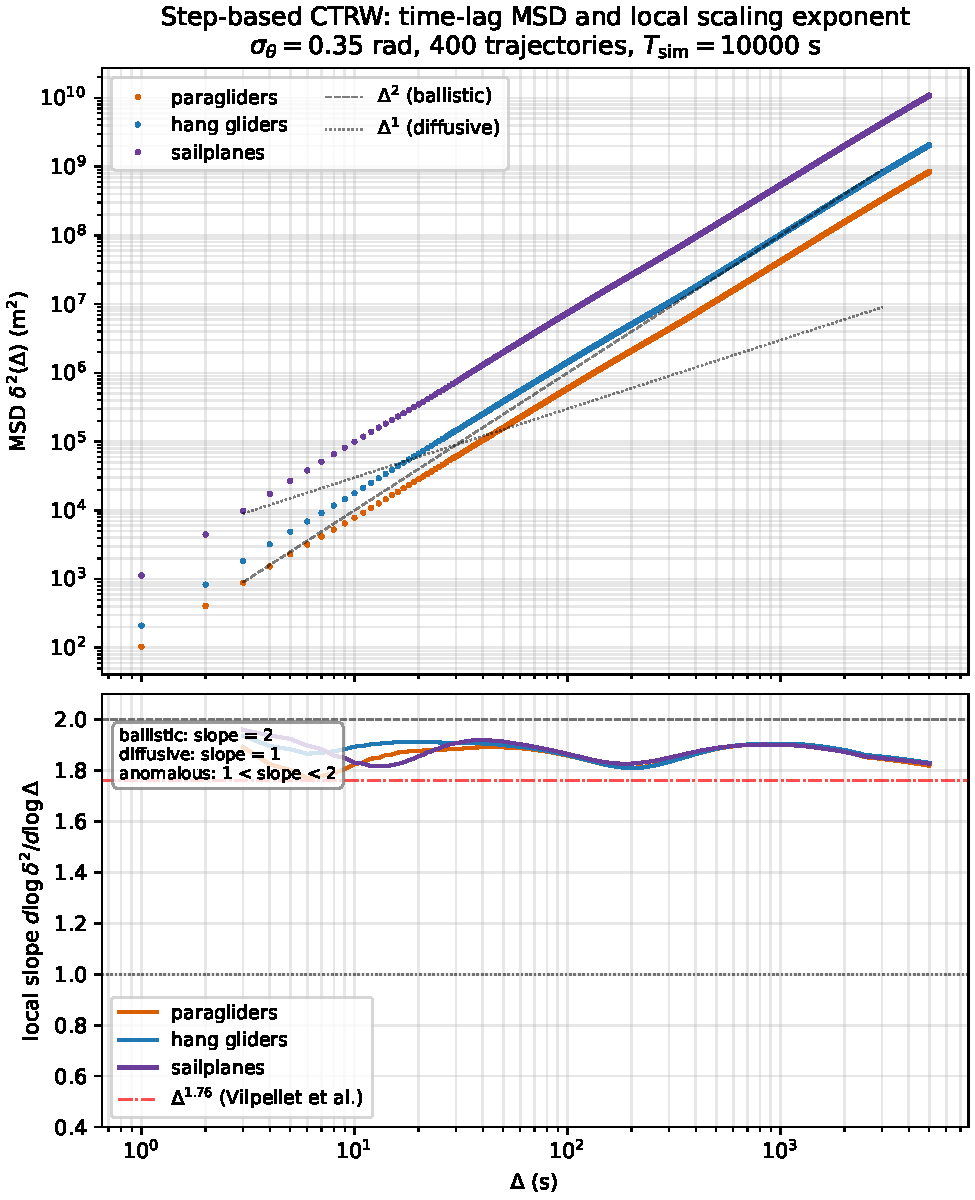
\includegraphics[width=0.95\columnwidth]{figures/local_slope_diagnostic.pdf}
\caption{\label{fig:local-slope}%
Local logarithmic slope of the simulated MSD,
$d\log\delta^2/d\log\Delta$, for the three aircraft. The slope
starts near the ballistic value $2$ at $\Delta\sim\langle T\rangle$
and decreases monotonically towards the diffusive value $1$ on a
scale $\simeq N_p\langle T\rangle$. Within the VDB window
$10<\Delta<5\times 10^3$\,s the curves traverse the
sub-ballistic range $[1.7,1.9]$, a signature of the pre-asymptotic
crossover. A genuine fBm/L\'evy-flight asymptotic origin of
$H=0.88$ would instead produce a \emph{constant} slope of $2H$
across this window. This discriminant diagnostic can be
straightforwardly computed on the empirical MSD
of~\cite{vilpellet2026}.}
\end{figure}

\paragraph*{Sensitivity and robustness.}
Two checks quantify how sharply the mechanism picks out
$\sigma_\theta\simeq 0.35$\,rad. (a) \emph{Sensitivity of $H_{\mathrm{eff}}$
to $\sigma_\theta$.} Reading the slope of the iso-$H$ contour of
Fig.~\ref{fig:phase} at the empirical $\mu_T$ values, we find
$|\partial H_{\mathrm{eff}}/\partial\sigma_\theta|\simeq 0.25\,
\mathrm{rad}^{-1}$ in the empirically relevant range; a $\pm 20\%$
change of $\sigma_\theta$ therefore shifts $H_{\mathrm{eff}}$ by
$\pm 0.02$ only, consistent with the tight aircraft-to-aircraft
spread $\Delta H\lesssim 0.01$ observed in the Monte Carlo runs.
(b) \emph{Physical interpretation of $N_p$.} The effective
persistence length in cycle units,
$N_p\simeq 16$ cycles, corresponds to
$N_p\langle T\rangle\simeq 6.8\times 10^3$\,s, \emph{i.e.}\
roughly two hours of continuous soaring. This is comparable to the
typical duration of a cross-country flight, which explains why
the empirical lag window of~\cite{vilpellet2026} exactly samples
the pre-asymptotic crossover and does not reach the diffusive
asymptote.

\paragraph*{Limitations and extensions.}
The present analysis makes three simplifying assumptions that
deserve comment. (a) The cycle-to-cycle heading increment
$\eta_n\sim\mathcal{N}(0,\sigma_\theta^2)$ is Gaussian and
i.i.d.; in reality pilots adapt their next heading to the search
outcome, which would introduce intra-cycle feedback. Allowing
$\sigma_\theta\to\sigma_\theta(n)$ to drift with experience is the
natural mechanism for the experience-dependent $H$ reported
in~\cite{vilpellet2026}. (b) The orographic drift
$v_{\mathrm{drift}}$ is treated as a constant vector shared by all
climbs of an aircraft; a more realistic treatment would correlate
the drift with mountain geometry or wind direction, but this does
not affect the universality mechanism because
$v_{\mathrm{drift}}\ll v_{xy}$. (c) The Mittag-Leffler waits in
the intermittent search phase reduce to Pareto waits when the
tail index satisfies $\alpha>1$; this is the regime sampled by all
three aircraft and no loss of generality is incurred. Natural
extensions of the model, all compatible with the present code
architecture, include: replacing the Gaussian angular increment
with a heavy-tailed one to alter the cycle-to-cycle heading
autocorrelation tail; adding a mean wind-drift term to separate
air-relative from ground-relative motion; and promoting
$\sigma_\theta$ to a pilot-specific adaptive parameter.

A longer companion manuscript, containing full derivations of
Eqs.~\eqref{eq:msd-search}--\eqref{eq:msd-N}, the complete set of
intra-phase calibration plots, and the simulation code, is
available from the author upon request.

\paragraph*{Acknowledgments.}
The author thanks M.~Benzaquen, D.~Challet and A.~Darmon for
making the motivating internship project openly
advertised~\cite{vilpellet2026}, and the EconophysiX Lab for the
scientific context of this work.

{\footnotesize
\bibliographystyle{unsrt}
\bibliography{references}
}

\end{document}
